\section{B-Tree}

\subsection{2-3 Tree}

\vspace{\parskip}

\begin{definition} \index{2-3 tree}
    A \textbf{search} tree is a 2-3 tree if every internal node has either two children with one element, or three children with two elements. Leaf nodes of a 2-3 tree have no children and one or two elements. More formally, a tree $T$  is a 2-3 tree if and only if one of the following is true:
    \begin{itemize}
        \item $T$ is empty
        \item $T$ has one element $a$ and two children $p,q$ ($p$ being the left child and $q$ being the right child). $p$ and $q$ are 2-3 trees of the same height, and $a$ is greater than every element in $p$, and $a$ is less than every element in $q$ 
        \item $T$ has two elements $a < b$ and three children $p,q,r$ (left, middle, right children, respectively). $p$ and $q$ are 2-3 trees of the same height; and $a$ is greater than every element in $p$ and less than every element in $q$; and $b$ is greater than every element in $q$ and less than every element in $r$.
    \end{itemize}
    \begin{center}
        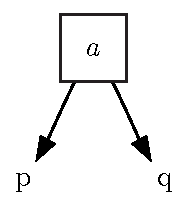
\includegraphics[width=0.15\linewidth]{2-3tree_2node.pdf} 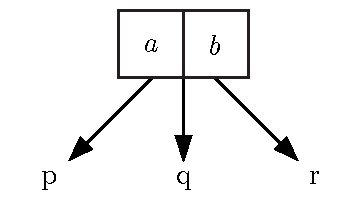
\includegraphics[width=0.3\linewidth]{2-3tree_3node.pdf}
    \end{center}
\end{definition}